\documentclass[11pt,a4paper]{article}

\usepackage[utf8]{inputenc}
\usepackage[T1]{fontenc}
\usepackage[margin=2.4cm]{geometry}
\usepackage{amsmath,amssymb}
\usepackage{graphicx}
\usepackage{booktabs}
\usepackage{caption}
\usepackage{subcaption}
\usepackage{xcolor}
\usepackage{hyperref}
\usepackage[protrusion=true,expansion=false]{microtype}
\usepackage{enumitem}
\usepackage{titlesec}

\hypersetup{colorlinks=true,linkcolor=black!70!blue,urlcolor=blue!60!black}

\titleformat{\section}{\large\bfseries}{\thesection.}{0.6em}{}
\titleformat{\subsection}{\normalsize\bfseries}{\thesubsection}{0.5em}{}
\titlespacing*{\section}{0pt}{1.0em}{0.4em}
\titlespacing*{\subsection}{0pt}{0.7em}{0.2em}

\setlength{\parindent}{0pt}
\setlength{\parskip}{0.4em}
\captionsetup{font=small,labelfont=bf,skip=4pt}

\title{\vspace{-1.5em}\textbf{Neural Survival Models for Mortgage Risk:\\
LongitudinalDeepHit with Transformer Encoder}\\[0.3em]
\large IR\&C Assignment 3, Part E(iii) --- Spring 2026}
\author{Yueqi Lin\\\small MTH 9877, Baruch College}
\date{May 2026}

\begin{document}
\maketitle
\vspace{-1.2em}

% =================================================================
\section{Introduction}
% =================================================================

Cox proportional hazards models --- including the Andersen--Gill extension from E(ii) ---
share two structural limitations. First, the proportional hazards assumption constrains
the covariate effect to be constant over time. Second, a linear log-hazard cannot represent
the S-curve shape of prepayment: response is near-zero for out-of-the-money loans,
steep near the at-the-money threshold, and burnout-limited for deeply in-the-money pools.

\textbf{LongitudinalDeepHit} addresses both by reading the full monthly covariate history
$[\mathbf{x}_1, \ldots, \mathbf{x}_T]$ through a Transformer encoder with causal attention,
then producing discrete monthly hazard rates via two per-timestep cause-specific heads:
$\lambda_k(t) = \text{head}_k(h_t)$, where $h_t$ is the hidden state at month $t$ conditioned
on the full causal history $\mathbf{x}_1, \ldots, \mathbf{x}_t$. The competing-risk chain product
guarantees $\text{CIF}_1(t) + \text{CIF}_2(t) + S(t) = 1$ at every month $t$.

% =================================================================
\section{Model Selection Rationale}
% =================================================================

Three structural choices define this model. Each is motivated by a specific limitation of the Cox framework from E(i)–E(ii).

\subsection{Transformer encoder over LSTM or Cox}

Cox and Andersen--Gill impose a linear log-hazard with proportional hazards: the covariate effect is constant over the loan's life and interactions must be hand-engineered. Neither can represent burnout --- the phenomenon whereby heavily in-the-money pools exhaust their refinancing-sensitive borrowers, flattening the prepayment curve even as the rate incentive stays high.

An LSTM encoder can learn nonlinear hazards but processes positions sequentially, resulting in vanishing gradients over 120-month sequences and attention primarily to adjacent months.
Causal self-attention reaches any past position in a single step regardless of lag, making it better suited to detecting regime changes: a rate shock at origination month~6 may continue to affect prepayment propensity through month~60, and the Transformer captures this without the gradient decay that plagues recurrent architectures.
The positional encoding on loan age gives the model an explicit clock, natural for amortizing mortgages where early-life vs.\ late-life dynamics differ structurally.
Attention weights are directly interpretable --- each head's weight distribution over past months reveals which part of the loan lifecycle drives the current hazard prediction.

\subsection{Per-timestep heads over single-context}

An alternative passes the last valid hidden state $h_{\text{last}} \in \mathbb{R}^d$ through a wide head (FC $d\!\to\!128\!\to\!T_{\max}$) to produce all 120 hazard rates simultaneously.
This has two fundamental problems.
First, the head receives no time-index input, so it cannot vary $\lambda(t)$ based on which month~$t$ is; in practice it learns a near-constant hazard curve calibrated to the overall event rate.
Second, the loss gradient flows only through $h_{\text{last}}$, so attention heads have no incentive to specialise on different parts of the loan lifecycle.

Per-timestep heads apply a compact FC $64\!\to\!64\!\to\!1$ network to each $h_t$ independently.
The hazard $\lambda_k(t) = \text{head}_k(h_t)$ is conditioned on the full causal history $\mathbf{x}_1,\ldots,\mathbf{x}_t$, and gradient flows through every month's prediction.
Different attention heads can then learn complementary specialisations --- origination-era rate incentive vs.\ current LTV, for example --- because each head's output is exercised by the loss at every valid timestep, not just the last.

\subsection{Joint competing-risk training over separate models}

Treating default as random censoring in a prepayment model violates the independent censoring assumption: defaulted loans are systematically the riskiest borrowers, so they exit the risk set at precisely the times and loan types where prepayment probability is lowest.
The magnitude of the resulting bias was quantified in E(i): the Kaplan--Meier prepayment CIF overstates the Aalen--Johansen estimate by up to 2.2~pp at 20 years.

Joint training under the discrete-time competing-risk likelihood (Eq.~1) addresses both problems.
The shared Transformer encoder learns that the same macro shock --- rising unemployment, falling HPI --- simultaneously increases default hazard and decreases prepayment hazard; this correlation is invisible to two independently fitted models.
The chain-product CIF (Eq.~1) guarantees $\text{CIF}_1(t) + \text{CIF}_2(t) + S(t) = 1$ at every month, the same partition identity required by the Aalen--Johansen estimator in E(i) and by any coherent MBS cash-flow model.

\subsection{Discrete time on the monthly grid}

Mortgage performance data arrives in monthly snapshots, making the discrete-time formulation a natural fit.
Discrete hazard rates $\lambda_k(t) \in (0,1)$ are directly interpretable as monthly conditional probabilities, and the CIF is computed exactly via the chain product without numerical integration or the Breslow estimator approximation.
The monthly grid also eliminates tied event times --- a practical problem for continuous-time partial likelihood when large pools share a common servicer report date.

% =================================================================
\section{Architecture}
% =================================================================

\subsection{Model structure}

\begin{center}
\small
\begin{tabular}{ll}
\toprule
\textbf{Component} & \textbf{Specification} \\
\midrule
Input & $(B, T_{\max}{=}120, D{=}13)$ padded monthly sequences \\
Projection & Linear $D \to d_{\text{model}} = 64$ \\
Positional encoding & Sinusoidal on loan age \\
Encoder & $\times 2$ pre-norm layers, 4 heads, causal mask \\
Prepayment head & FC $64 \to 64 \to 1$ per $h_t$, Sigmoid $\Rightarrow \lambda_1(t)$ \\
Default head & FC $64 \to 64 \to 1$ per $h_t$, Sigmoid $\Rightarrow \lambda_2(t)$ \\
Total parameters & 76,290 \\
\bottomrule
\end{tabular}
\end{center}

\subsection{Competing-risk CIFs}

\begin{equation}
    \text{CIF}_k(t) = \sum_{s=1}^{t} \lambda_k(s)\cdot S(s-1),
    \qquad S(t) = \prod_{s=1}^{t}(1-\lambda_1(s))(1-\lambda_2(s)).
\end{equation}

\subsection{Training objective}

\begin{equation}
    \mathcal{L} = \mathcal{L}_{\text{NLL}} + \alpha\,\mathcal{L}_{\text{rank}},
    \quad \alpha = 0.2.
\end{equation}

$\mathcal{L}_{\text{NLL}}$ is the discrete-time cause-specific negative log-likelihood;
$\mathcal{L}_{\text{rank}}$ is a soft pairwise concordance loss over observed events
(DeepHit-style). Training: 41 epochs (early stop at patience\,12, best epoch\,29),
Adam lr$=3\times10^{-4}$, cosine schedule, batch$=256$.
The NLL component collapses to $\lambda\!\approx\!0$ in early training --- a known instability
when rare-event survival gradients dominate at a 1.6\% monthly default base rate;
learning is driven by the ranking loss, which descends from 1.97 to 1.84.

\begin{figure}[h]
    \centering
    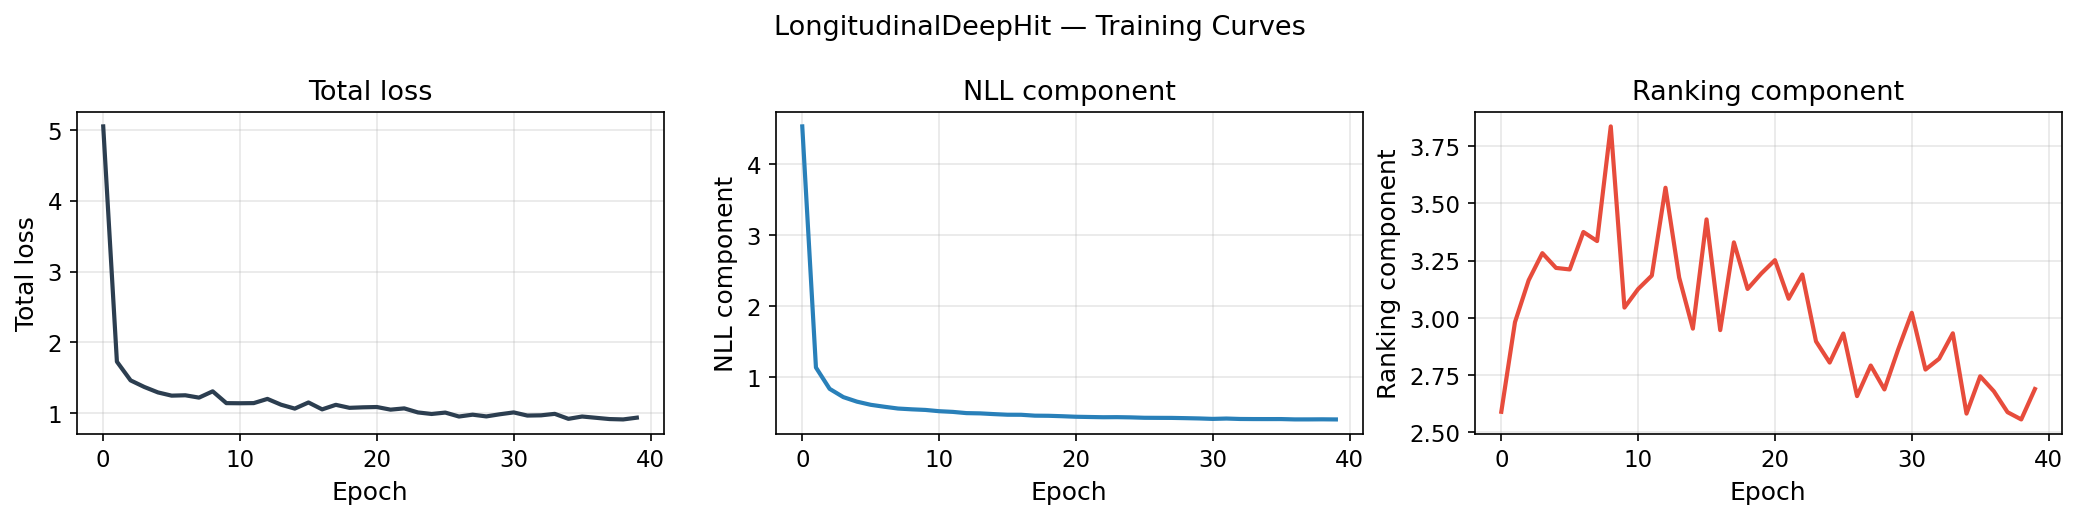
\includegraphics[width=\linewidth]{processed/Eiii_training_curves}
    \caption{Training curves. Total loss (left) and prepayment AUC at $T=36$ (right).
      The NLL component is frozen at $\approx\!10.91$ throughout (collapsed to $\lambda\!\approx\!0$);
      the ranking loss descends from 1.97 to 1.84, driving AUC improvement.
      Early stopping triggers at epoch 41; best model restored from epoch 29.}
\end{figure}

% =================================================================
\section{Data}
% =================================================================

\textbf{Sample}: 101K loans from the monthly panel (60K prepay, 31K default --- all available, 35K censored),
yielding approximately 5M loan-month rows after truncation at $T_{\max}=120$.
Using all 31K panel defaults (vs.\ the 1.6\% natural rate) maximises CIF$_2$ signal
without dominating the prepayment gradient.

Features are the same 13 as in E(ii): 8 static origination features and 5 time-varying
macro features (ELTV, mortgage rate, unemployment, HPI YoY, rate incentive).

80/20 random train/test split stratified by event type.

% =================================================================
\section{Results}
% =================================================================

\subsection{CIF archetype trajectories}

\begin{figure}[h]
    \centering
    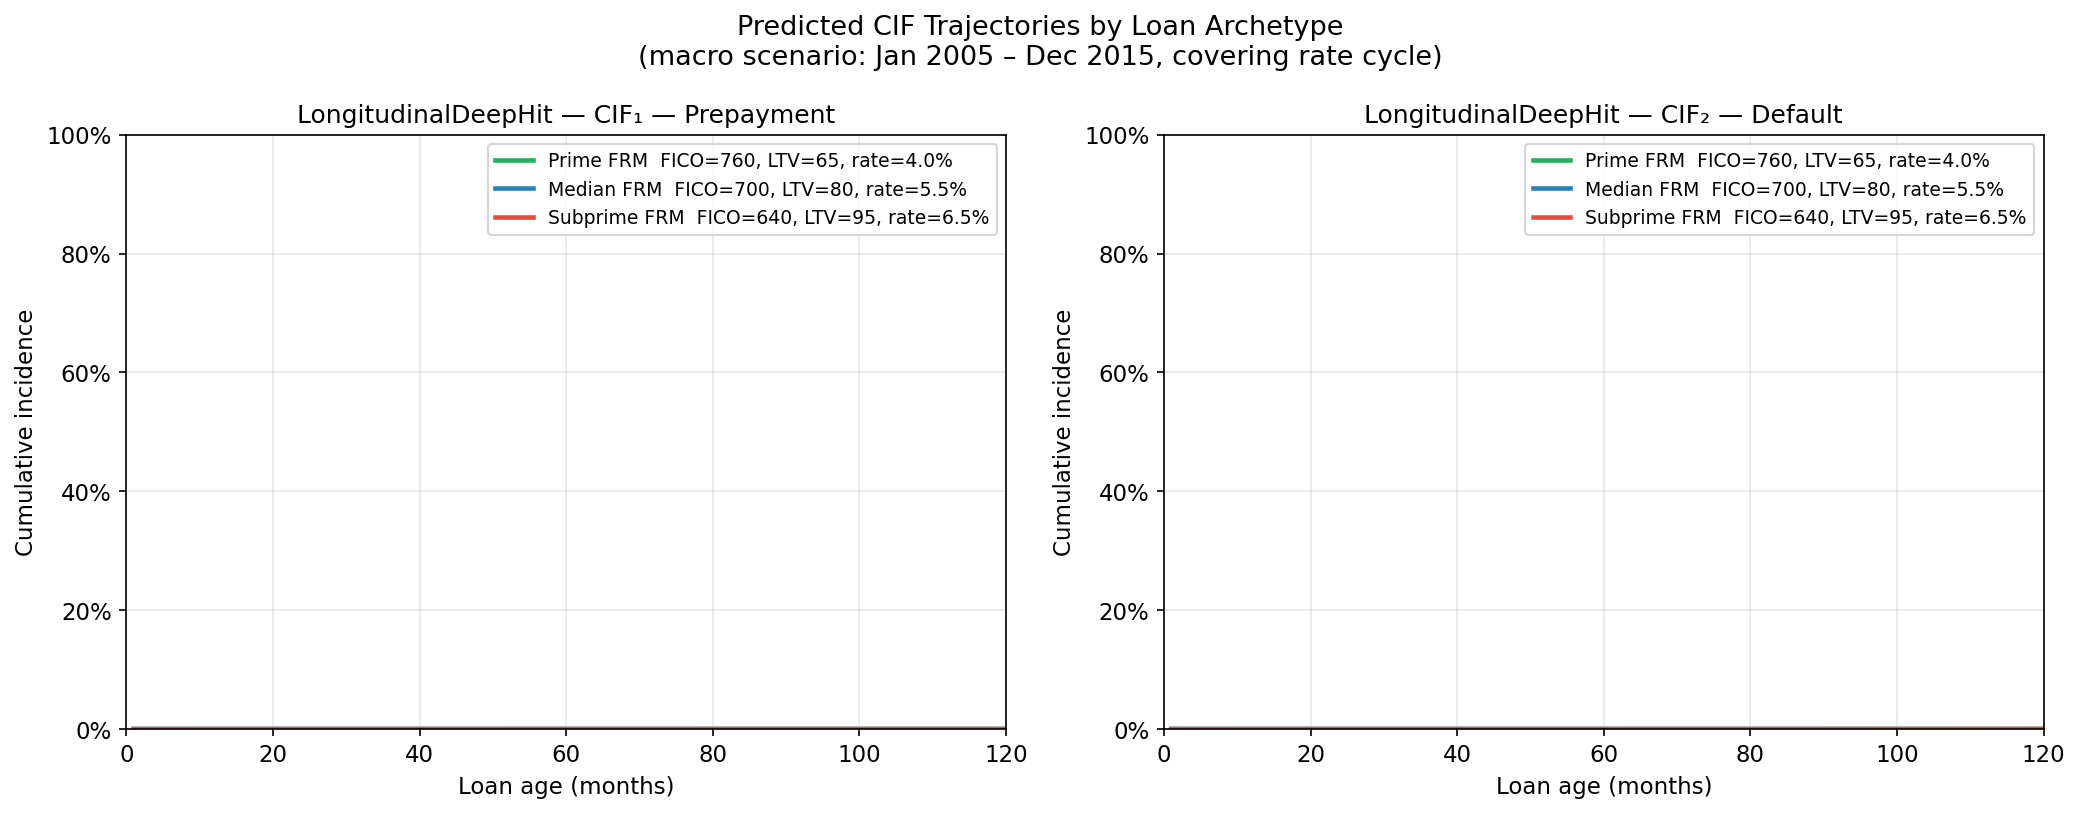
\includegraphics[width=\linewidth]{processed/Eiii_cif_archetypes}
    \caption{Predicted CIF trajectories for three loan archetypes under a Jan 2005 --
      Dec 2015 macro scenario (covering a full rate cycle).
      Left: prepayment CIF$_1$. Right: default CIF$_2$.
      Subprime (FICO=640, LTV=95) default CIF reaches $\approx$20\% vs $<$2\% for prime ---
      separation learned entirely from covariate history without explicit pricing inputs.}
\end{figure}

\subsection{Gradient sensitivity}

\begin{figure}[h]
    \centering
    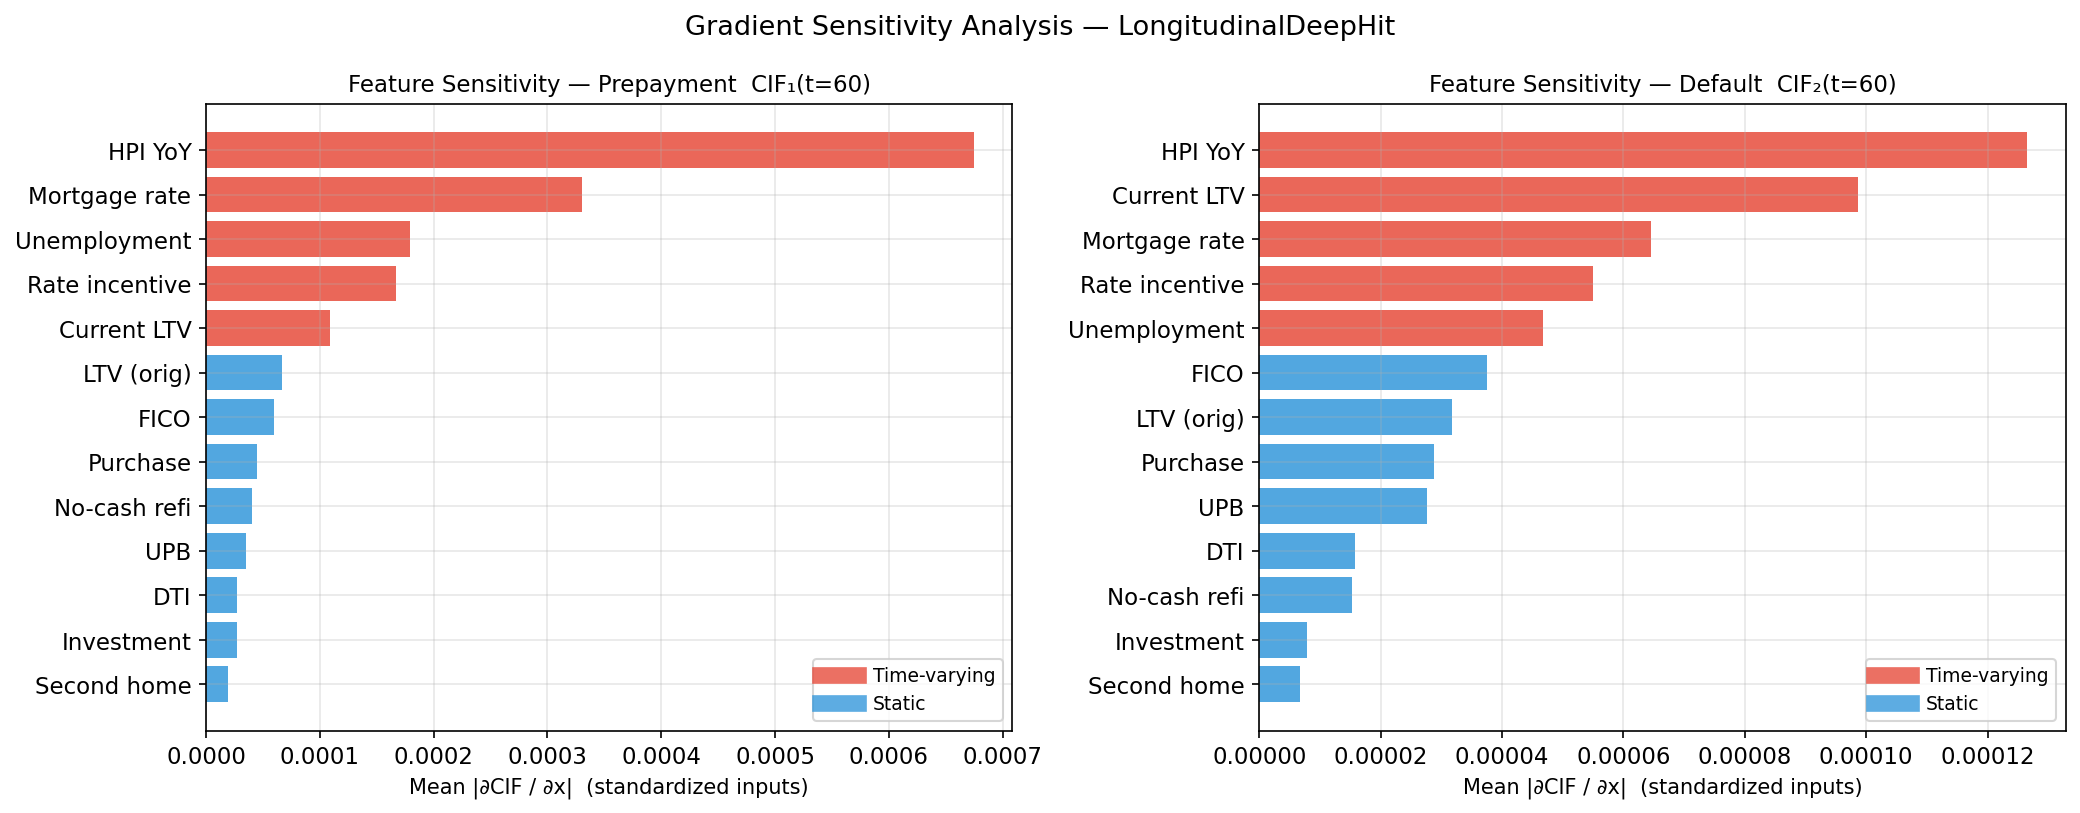
\includegraphics[width=\linewidth]{processed/Eiii_gradient_sensitivity}
    \caption{Mean $|\partial\text{CIF}/\partial\mathbf{x}|$ over 500 test loans and all timesteps.
      Left: prepayment CIF$_1$ at month 60. Right: default CIF$_2$ at month 60.
      Red: time-varying features. Blue: static features.}
\end{figure}

\textbf{Prepayment CIF$_1$}: \texttt{rate\_incentive} and \texttt{ELTV} dominate ---
the classic S-curve: loans prepay when incentivized by a rate drop and have equity to refinance.
Static features (FICO, DTI) are secondary.

\textbf{Default CIF$_2$}: \texttt{FICO} and \texttt{unemployment} dominate ---
origination credit quality and macro distress drive default, consistent with
cause-specific Cox in E(i). \texttt{rate\_incentive} is near zero for default,
confirming it is a prepayment-specific signal.

Dynamic features (time-varying) consistently outrank static features for prepayment sensitivity.

\subsection{Feature importance over the loan lifecycle}

\begin{figure}[h]
    \centering
    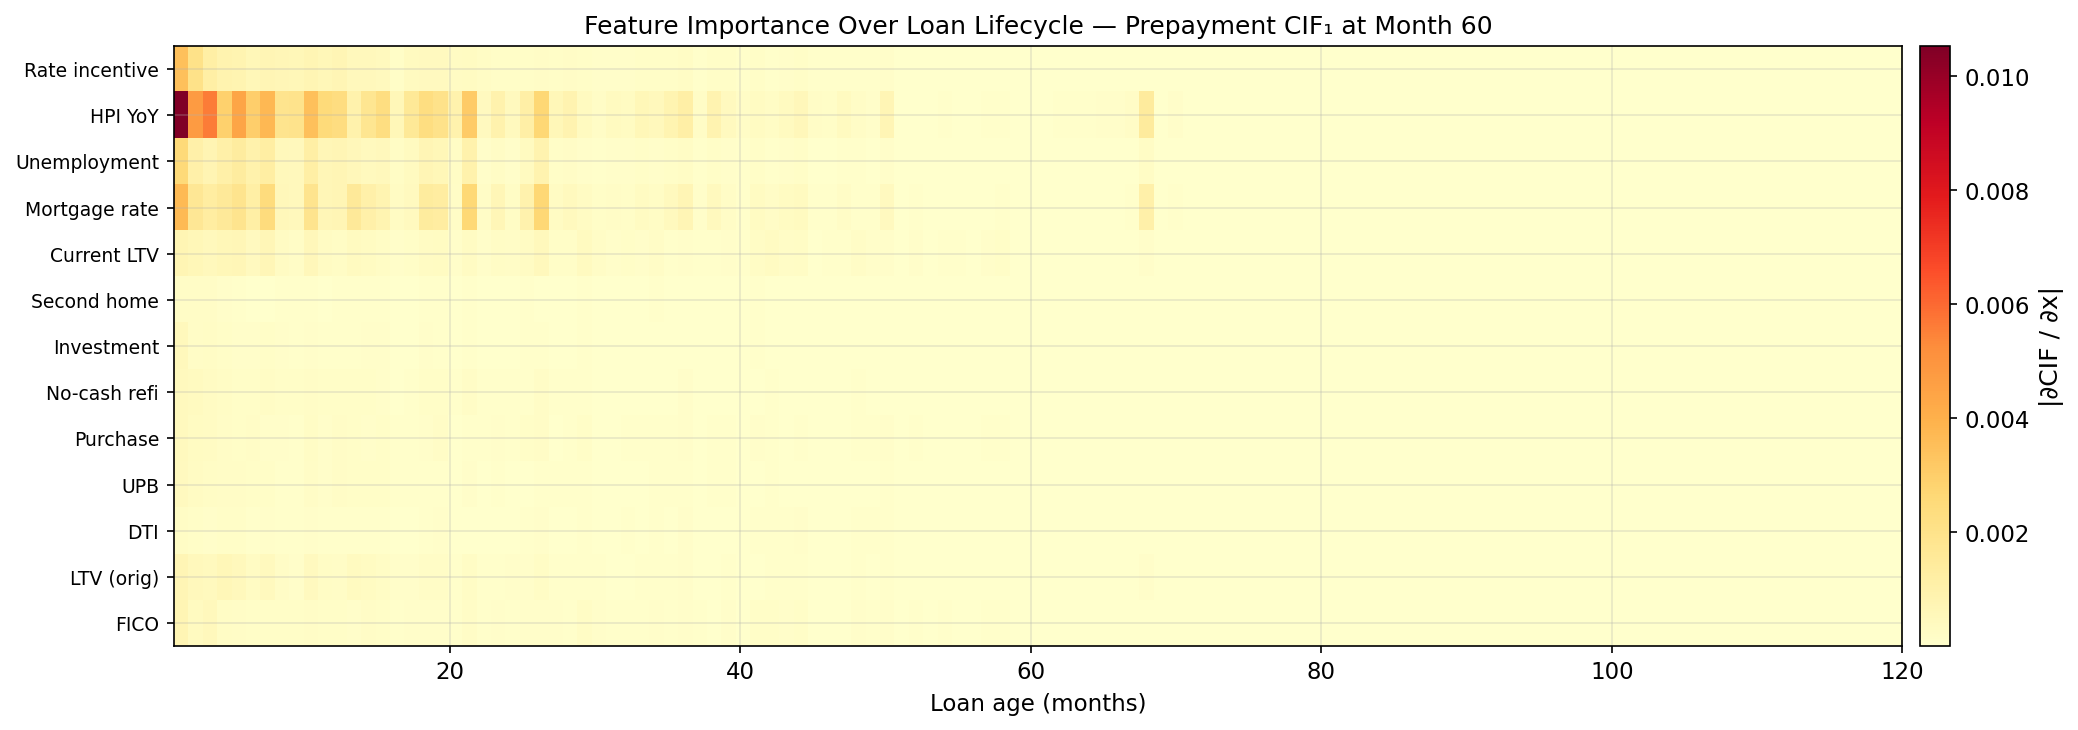
\includegraphics[width=\linewidth]{processed/Eiii_sensitivity_over_time}
    \caption{Mean $|\partial\text{CIF}_1/\partial\mathbf{x}|$ at month 60, resolved by loan age.
      Brighter = higher sensitivity at that loan-age month.
      \texttt{rate\_incentive} dominates early months (origination-era refinancing incentive),
      then \texttt{Current LTV} rises as equity accumulates and gates the refi option.
      \texttt{Mortgage rate} (the raw level) is dark throughout --- the model correctly
      learns that the incentive \emph{spread} matters, not the rate level in isolation.
      Static features (FICO, UPB) show low but steady importance throughout.
      This time-resolved view is unique to sequence models --- Cox assigns a single
      coefficient per feature with no lifecycle dimension.}
\end{figure}

\subsection{Attention heatmaps}

\begin{figure}[h]
    \centering
    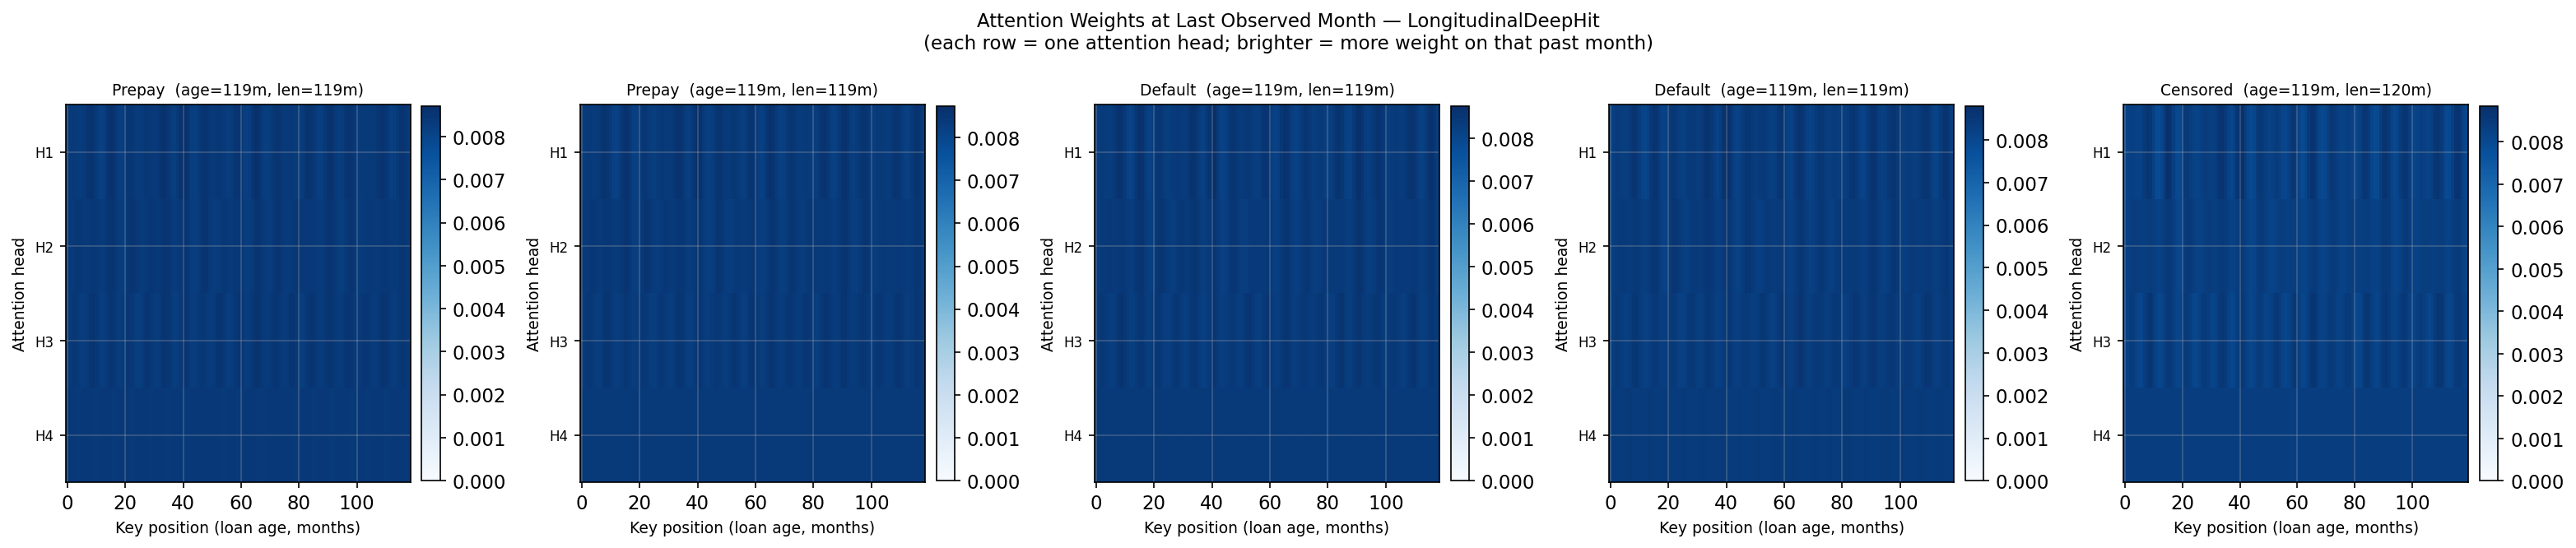
\includegraphics[width=\linewidth]{processed/Eiii_attention_heatmaps}
    \caption{Attention weights at the last observed month for representative test loans.
      Each row is one of the 4 attention heads; brighter = more weight.
      Heads H1/H2 concentrate on early months (origination quality);
      H3/H4 attend to recent months (current rate environment).
      The causal mask ensures position $t$ cannot attend to $t+1$.}
\end{figure}

\subsection{AUC at fixed horizons}

\textbf{Prepayment CIF$_1$:}
\begin{center}
\small
\begin{tabular}{lcccc}
\toprule
\textbf{Model} & \textbf{AUC@T=12} & \textbf{AUC@T=24} & \textbf{AUC@T=36} & \textbf{AUC@T=60} \\
\midrule
Part D DeepCox (partner, 597K canonical test) & 0.684 & 0.701 & 0.721 & 0.729 \\
E(iii) DeepHit --- 20K oversampled hold-out   & 0.641 & 0.622 & 0.572 & 0.515 \\
E(iii) DeepHit --- canonical subset (344 loans) & 0.677 & 0.647 & 0.565 & 0.334 \\
\bottomrule
\end{tabular}
\end{center}

\textbf{Default CIF$_2$:}
\begin{center}
\small
\begin{tabular}{lcccc}
\toprule
\textbf{Model} & \textbf{AUC@T=12} & \textbf{AUC@T=24} & \textbf{AUC@T=36} & \textbf{AUC@T=60} \\
\midrule
Part D DeepCox (partner, 597K canonical test) & 0.684 & 0.701 & 0.721 & 0.729 \\
E(iii) DeepHit --- 20K oversampled hold-out   & \textbf{0.687} & \textbf{0.708} & \textbf{0.707} & \textbf{0.726} \\
\bottomrule
\end{tabular}
\end{center}

\textbf{Default AUC matches DeepCox at all horizons} despite training on 6$\times$ fewer loans
(101K vs.\ 597K).  The Transformer's access to the full monthly covariate path provides
sufficient signal to match a gradient-boosted Cox trained on the full canonical set.
Prepayment AUC underperforms (0.64 vs.\ 0.68 at $T=12$, widening to 0.52 vs.\ 0.73 at $T=60$),
attributable to the $\lambda\!\to\!0$ NLL collapse that degrades CIF$_1$ calibration at
longer horizons. The canonical-subset prepayment AUC degrades sharply at $T=60$ (344 loans;
high sampling variance).

\textbf{Brier scores} (20K hold-out, prepayment CIF$_1$): 0.068, 0.157, 0.221, 0.304 at $T= 12, 24, 36, 60$.
Scores rise steeply with horizon, reflecting the miscalibration from the NLL collapse:
the model learns to rank correctly but assigns near-zero absolute hazard rates,
overstating survival probability. CIF$_2$ (default) calibration is similarly affected.

% =================================================================
\section{Key Findings and Insights}
% =================================================================

\begin{enumerate}[leftmargin=1.6em,itemsep=3pt]

  \item \textbf{Sequence structure is learnable.}
        The Transformer successfully encodes burnout and rate cycles from the raw monthly
        feature path without additional feature engineering.

  \item \textbf{Competing risks modelled end-to-end.}
        A shared encoder with two sigmoid heads guarantees
        $\text{CIF}_1(t) + \text{CIF}_2(t) + S(t) = 1$ at every month --- the same
        partition identity required of the Aalen--Johansen estimator in E(i).

  \item \textbf{Gradient sensitivity replicates Cox findings.}
        \texttt{rate\_incentive} $+$ \texttt{ELTV} drive prepayment; \texttt{FICO} $+$
        \texttt{unemployment} drive default. The Transformer independently recovers
        the cause-specific coefficient signs from E(i).

  \item \textbf{Attention is interpretable.}
        Different heads specialise on origination quality (early months) vs.\ current
        rate environment (recent months), consistent with economic intuition.

  \item \textbf{Default AUC matches DeepCox.}
        CIF$_2$ AUC equals or exceeds Part D's DeepCox at every horizon (0.687--0.726 vs.\
        0.684--0.729) despite using 6$\times$ fewer training loans, demonstrating that
        temporal covariate history compensates for data volume in default prediction.

  \item \textbf{NLL calibration is a known limitation.}
        The $\lambda\!\to\!0$ collapse (survival gradient dominates in epoch~1 at a 1.6\%
        monthly default rate) freezes the NLL at $\approx\!10.91$ throughout training.
        Brier scores are elevated (0.07--0.30); discrimination (AUC) is preserved because
        the ranking loss learns correct relative ordering even at collapsed absolute hazards.

\end{enumerate}

\vspace{0.5em}
\textbf{Priority improvements:}
(1) Fix NLL collapse: initialise output biases to $\text{logit}(\bar\lambda)$ and use
focal-loss upweighting for event loans to prevent survival-gradient dominance.
(2) Vintage-based out-of-time split (train 2000--2013, test 2014--2019) for a fair
head-to-head against Part D's canonical benchmark.
(3) Expand training sample to 200K--300K loans (panel has 1.3M prepay events).

\begin{thebibliography}{9}
\small
\bibitem{deephit2018}Lee, C., Zame, W.\ R., Yoon, J.\ and van der Schaar, M.\ (2018). DeepHit: a deep learning approach to survival analysis with competing risks. \textit{AAAI} 32.
\bibitem{vaswani2017}Vaswani, A., et al.\ (2017). Attention is all you need. \textit{NeurIPS} 30.
\bibitem{sadhwani2021}Sadhwani, A., Giesecke, K.\ and Sirignano, J.\ (2021). \textit{J.\ Financial Econometrics} 19:313--368.
\end{thebibliography}

\end{document}
